% ********************************** CHAPTER 3 source ***********************************************




%%%%%%%%%%%%%%%%%%%%%%%%%%%%%%%%%%%%%%%%%%%%%%%%%%%%%%%%
\section{Teoretický popis funkce vysílače} %%%%%%%%%%%%%%%%%%%%%%%%%%%%%%%%%%%%

Předpokládejme, že systém bude vysílat předem známou -- definovanou posloupnost bitů: $b(n)$ 
\begin{equation}
 b(n) = {b_0,b_1,\ldots,b_N} \label{eq:bseq}
\end{equation}
Známe jednak celkovou délku posloupnosti -- $N$ bitů a také hodnotu každého z bitů posloupnosti $b(n)$, přičemž $n$ je z oboru přirozených čísel. 


%%%%%%%%%%%%%%%%%%%%%%%%%%%%%%%% Modulation
\subsection{Moduační schéma}
\marginpar{\textcolor{txt_blue}{M-stavová modulace}}
Použita bude jednoduchá digitální modulace bez paměti (\textsl{angl.} memoryless), kdy je posloupnost bitů $b(n)$ mapována na jednotlivé symboly z M-prvkové množiny (\textsl{v angl. literatuře} M-ary mapping schema). Zvolená modulace je potom pojmenováne podle počtu dostupných symbolů "M-stavová". Podrobněji viz např. \cite{lathi2009}, \cite{proakis2007} nebo jiná literatura věnující se základům digitální modulace signálů. Posloupnost $b(n)$ je tudíž rozděnena na skupinky bitů o délce $k$, kde  
\begin{equation}
 k = \log_2M.  \label{eq:kfromM}
\end{equation}
Potom se z posloupnosti bitů $b(n)$, viz rovnice (\ref{eq:bseq}), stává posloupnost symbolů $a(l)$
\begin{equation}
 a(l) = {a_0,a_1,\ldots,a_L} \label{eq:sseq}
\end{equation}
Délka posloupnosti symbolů je $L$, kdy $L=\frac{N}{k}$.

\marginpar{\textcolor{txt_blue}{Bandpass signál}}
Každý \textsl{symbol} $a(l)$, který je tvořen skupinkou $k$ bitů je mapován na jeden z $M$ možných signálů $s_m(t)$ (\textsl{angl.} waveforms). 
\begin{equation}
 s_m(t), 1 \leq m \leq 2^k.  \label{eq:waveforms}
\end{equation}

Jedná se o harmonické signály tzv. vysokofrekvenční (VF), tedy fakticky o signály v podobě, v jaké budou vysílány anténou vysílače (\textsl{angl.} bandpass). Ty jsou charakteristické (a jedinečné) svou amplitudou, fází nebo svým kmitočtem, podle typu modulace. 

V této práci se budeme zabývat převážně signály, u nichž je modulovaná jejich fáze (\textsl{angl.}  phase--type of modulation). Podle \cite{proakis2007} je takový signál analyticky vyjádřen:
\begin{equation}
 s_m(t) = h(t)\cdot e^{j\frac{2\pi (m-1)}{M}} \cdot e^{j2\pi f_c t}.  \label{eq:waveformsBP}
\end{equation}

V tuto chvíli je možné $h(t)$ považovat za konstantu, která se v průběhu trvání jednoho symbolu nemění. Prostřední člen, který charakterizuje daný symbol, vyjádříme v exponenciálním tvaru:
\begin{equation}
 e^{j\frac{2\pi (m-1)}{M}} = \cos(2\pi \frac{m-1}{M}) + j\sin(2\pi \frac{m-1}{M}). \label{eq:waveformsBB00}
\end{equation}

\marginpar{\textcolor{txt_blue}{Baseband signál}}
Jak bylo naznačeno v předchozí kapitole, signály zastupující jednotlivé symboly, tedy \textsl{bandpass} signály mohou být reprezentovány jinými - nízkofrekvenčními signály tzv. základního pásma (\textsl{angl.} baseband). Ten je složen ze symfázní složky (\textsl{angl} in-phase) $s_m^I(t)$ a kvadraturní složky (\textsl{angl.} quadrature) $s_m^Q(t)$ podle:
\begin{equation}
 s_m^I(t) = h(t) \cdot \cos(2\pi \frac{m-1}{M}), \label{eq:waveformsI}
\end{equation}
\begin{equation}
 s_m^Q(t) = h(t) \cdot \sin(2\pi \frac{m-1}{M}). \label{eq:waveformsQ}
\end{equation}

Transformace signálu základního pásma na signál VF je realizována pomocí kvadraturního modulátoru (\textsl{angl.} quadrature modulation), viz např. \cite{proakis2007}. 


\subsection{Tvarování impulzu}
Každý ze symbolů posloupnosti $a(l)$ je vysílán po omezenou dobu. Po dobu trvání toho symbolu je vysílán patřičný signál $s_m$, který je v našem případě harmonický signál s příslušnou fází. V dalším textu budou tyto časové úseky nazývány v souladu s zaběhnutou terminologií impulzy. 

Pokud je, jak jsme doposud uvažovali, hodnota $h(t)$ po dobu celého jednoho impulzu konstantní, je okamžitá úroveň signálu základního pásma (jeho I a Q složky) dána hodnotou $m$, viz rovnice (\ref{eq:waveformsI}) a (\ref{eq:waveformsQ}). Pak mluvíme o obdélníkových impulzech (\textsl{angl} rectangular).

Z toho je zřejmé, že funkce $h(t)$ definuje tvar použitého impulzu. Jak bylo již zmíněno v úvodní části, není použití obdélníkových impulzů vždy výhodné vzhledem k jejich nekonečně širokému kmitočtovému spektru. Je běžnou praxí použít jiné -- výhodnější -- funkce pro $h(t)$ než je konstanta, a to například funkci \textsl{raised--cosine}:
 \begin{equation}
 h(t) =  \frac{\sin(\frac{\pi t}{T})}{\frac{\pi t}{T}}\cdot \frac{\cos(\pi \beta \frac{t}{T})}{1-4 \beta^2 (\frac{t}{T})^2}, \label{eq:pulseRC}
\end{equation}
kde $\beta$, z intervalu $0\leq \beta \leq 1$, je tzv. \textsl{roll-off} faktor. Detailněji viz \cite{lathi2009} nebo \cite{proakis2007}. Raised--cosine pulzy pro různé hodnoty $\beta$ jsou znázorněny na obr. \ref{fig:pulse_RCbeta}. Vězte, že pokud $\beta = 0$ potom $h(t)$ přechází na funkci $sinc(\pi t / T)$.

\begin{figure}[!t]
  \centering
  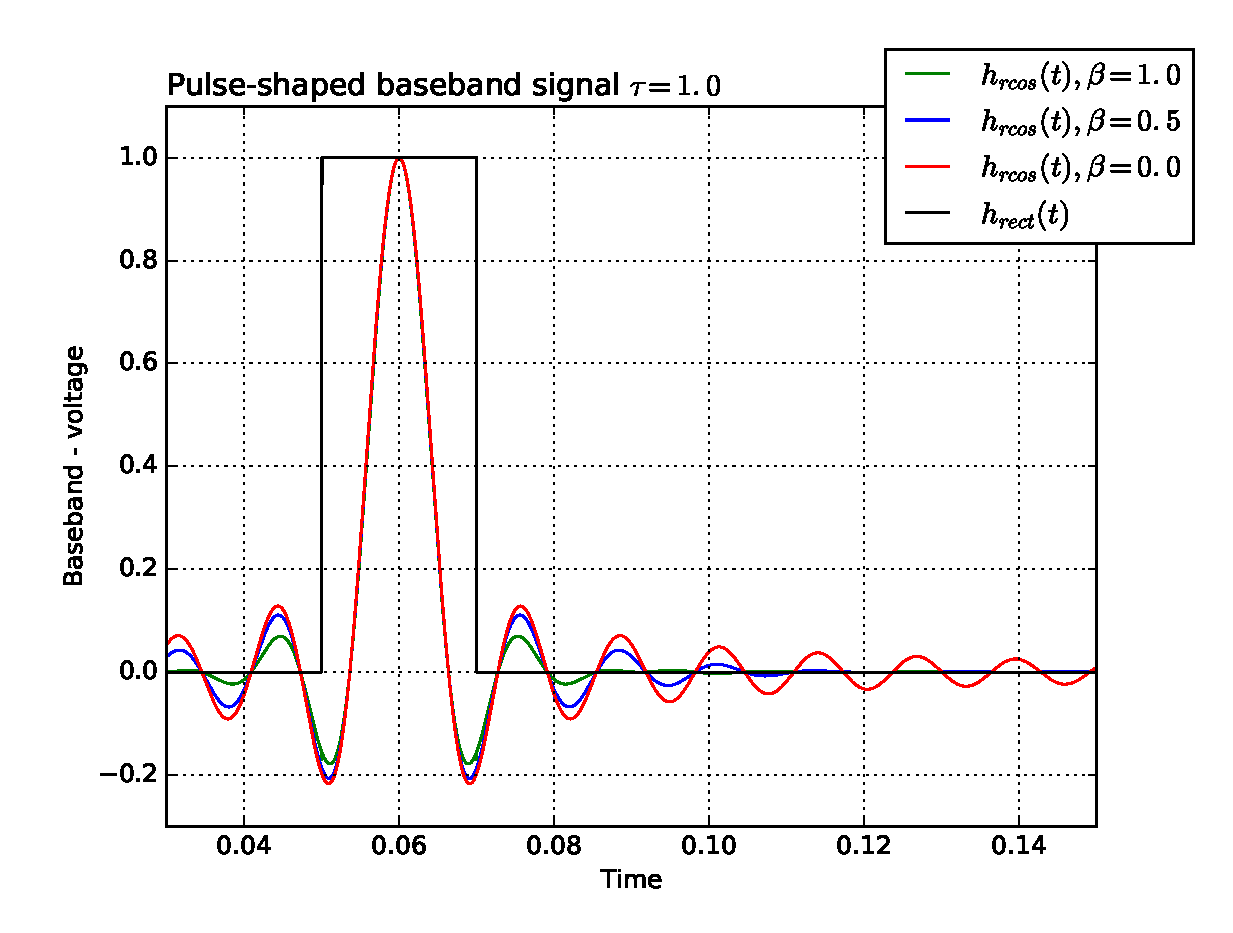
\includegraphics[width=3.5in]{./ch_03/img/Pulse_shaping_1.eps}
  \hfil
  \caption{Raised-cosine impulzy s rozdílnou hodnotou roll-off faktoru $\beta$.\label{fig:pulse_RCbeta}}
\end{figure}

%%%%%%%%%%%%%%%%%%%%%%%%%%%%%%%%%%%%% Timing
\subsection{Popis časových souvislostí signálu s tvarovaným impulzem}
Každý ze signálů $s_m(t)$ je vysílán po dobu trvání jednoho symbolu $T_s$ (\textsl{angl.} symbol interval). Odtud také symbolová rychlost $R_s$ (\textsl{angl.} symbol rate): 
\begin{equation}
 R_s = \frac{1}{T_s}  \label{eq:symrate}
\end{equation}

Potom $T_s$ definuje délku trvání impulzu a každý ze signálů $s_m(t)$ je vysílán uvnitř příslušného symbolového intervalu $T_s$ s patřičnou hodnotou parametru $m$. Tvarovací funkce  $h(t)$ z rovnice. (\ref{eq:pulseRC}) se tudíž mění na:
 \begin{equation}
 h(t-lT_s) =  \frac{\sin(\frac{\pi (t-lT_s)}{T_s})}{\frac{\pi (t-lT_s)}{T_s}}\cdot \frac{\cos(\pi \beta \frac{(t-lT_s)}{T_s})}{1-4 \beta^2 (\frac{(t-lT_s)}{T_s})^2}, \label{eq:pulseRCTs}
\end{equation}
kde $l$ značí pořadové číslo aktuálního symbolu v rámci posloupnosti $a(l)$.

Impuls tohoto tvaru potom splňuje Nyquistovo kritérium, viz \cite{proakis2007}, a nedochází k mezisymbolové interferenci (\textsl{angl} inter--symbol interference) a k nejednoznačnosti při detekci a identifikaci symbolu v přijímači.

Signál základního pásma pro příslušný $l$-tý symbol posloupnosti $a(l)$, potom z rovnice (\ref{eq:sseq}) je dán: 
\begin{equation}
 s_{m,l}^I(t) = h(t-lT_s) \cdot \cos(2\pi \frac{m_l-1}{M}), \label{eq:sigBBI}
\end{equation}
\begin{equation}
 s_{m,l}^Q(t) = h(t-lT_s) \cdot \sin(2\pi \frac{m_l-1}{M}). \label{eq:sigBBQ}
\end{equation}



